\chapter{Introducción}

Los sistemas de adquisición de datos (DAQs) son un conjunto de herramientas utilizadas para recopilar, procesar y analizar datos de fenómenos físicos. Los elementos básicos de un sistema de adquisición de datos incluyen sensores que capturan señales físicas, hardware de acondicionamiento de señales para procesar las salidas de los sensores, y una computadora que ejecuta software para adquirir y registrar los datos. 


El concepto de adquisición de datos se remonta a tiempos antiguos, cuando los seres humanos comenzaron a observar y registrar eventos naturales, como el movimiento de los cuerpos celestes, los cambios en el clima y el paso del tiempo. Las primeras civilizaciones desarrollaron métodos para la recolección de datos, como calendarios, instrumentos mecánicos, como el reloj solar, y libros de registros. Con la llegada de dispositivos analógicos y digitales, la adquisición de datos se hizo cada vez más sistemática y automatizada.


Algunos ejemplos de los sistemas de adquisición de datos aplicados en distintos sectores son: estaciones meteorológicas, utilizan DAQs para monitorear parámetros ambientales como la temperatura, la humedad, la velocidad del viento y la presión atmosférica. Estos sistemas suelen incluir sensores como termómetros, higrómetros y anemómetros, los datos se procesan y registran en ordenadores para hacer un seguimiento de los cambios climáticos. En la medicina, los electrocardiógrafos son un tipo de DAQs, miden la actividad eléctrica del corazón, procesan las señales y las muestran en forma de ondas en una pantalla. En la industria automotriz, durante la fase de desarrollo de los vehículos, los DAQs monitorean parámetros como el rendimiento del motor, la eficiencia del combustible y las emisiones de gases para garantizar el cumplimiento en los estándares de calidad y seguridad.


El uso de DAQs para la creación de imágenes con detectores infrarrojos, tiene múltiples aplicaciones, que van desde la seguridad y vigilancia en hogares \cite{Yii2023} hasta el ámbito médico, donde se utilizan para el diagnóstico de enfermedades como el cáncer de mama, diabetes \cite{LeneroBardallo2022} y patologías dermatológicas \cite{She2024}. También se emplean en la detección de gestos para dispositivos inteligentes \cite{LeBa2019} y en aplicaciones espaciales, como el monitoreo de las emisiones de dióxido de carbono en la atmósfera provocadas por la actividad humana \cite{Minoglou2019}. En la agricultura, para identificar las zonas del campo que sufren estrés hídrico o exceso de riego, lo que permite una mejor gestión del agua \cite{Parihar2021}.


Los detectores infrarrojos permiten capturar radiación que no es visible al ojo humano y la transforman en señales eléctricas que pueden ser medidas. Desarrollar un sistema de adquisición de datos para obtener imágenes infrarrojas es crucial, ya que estos sistemas interpretan las señales generadas por los detectores y las convierten en una imagen visible, proporcionando información valiosa sobre la distribución de la temperatura en un escenario específico.


Debido a la importancia de los sistemas de adquisición de datos en aplicaciones que utilizan detectores infrarrojos, es fundamental comprender el comportamiento de estos detectores. Conocer cómo responden a diferentes condiciones de luz y temperatura permite diseñar sistemas más eficientes y precisos para capturar imágenes térmicas.
    
    \section{Radiación Electromagnética}
    La radiación electromagnética es la emisión y transmisión de energía en forma de ondas electromagnéticas. El espectro electromagnético es una representación de los diversos tipos de radiación existentes, en él se definen los intervalos de longitudes de onda o frecuencia que cada una de ellas abarca \cite{Chang}.
            \begin{figure}[hbtp]
                \centering
                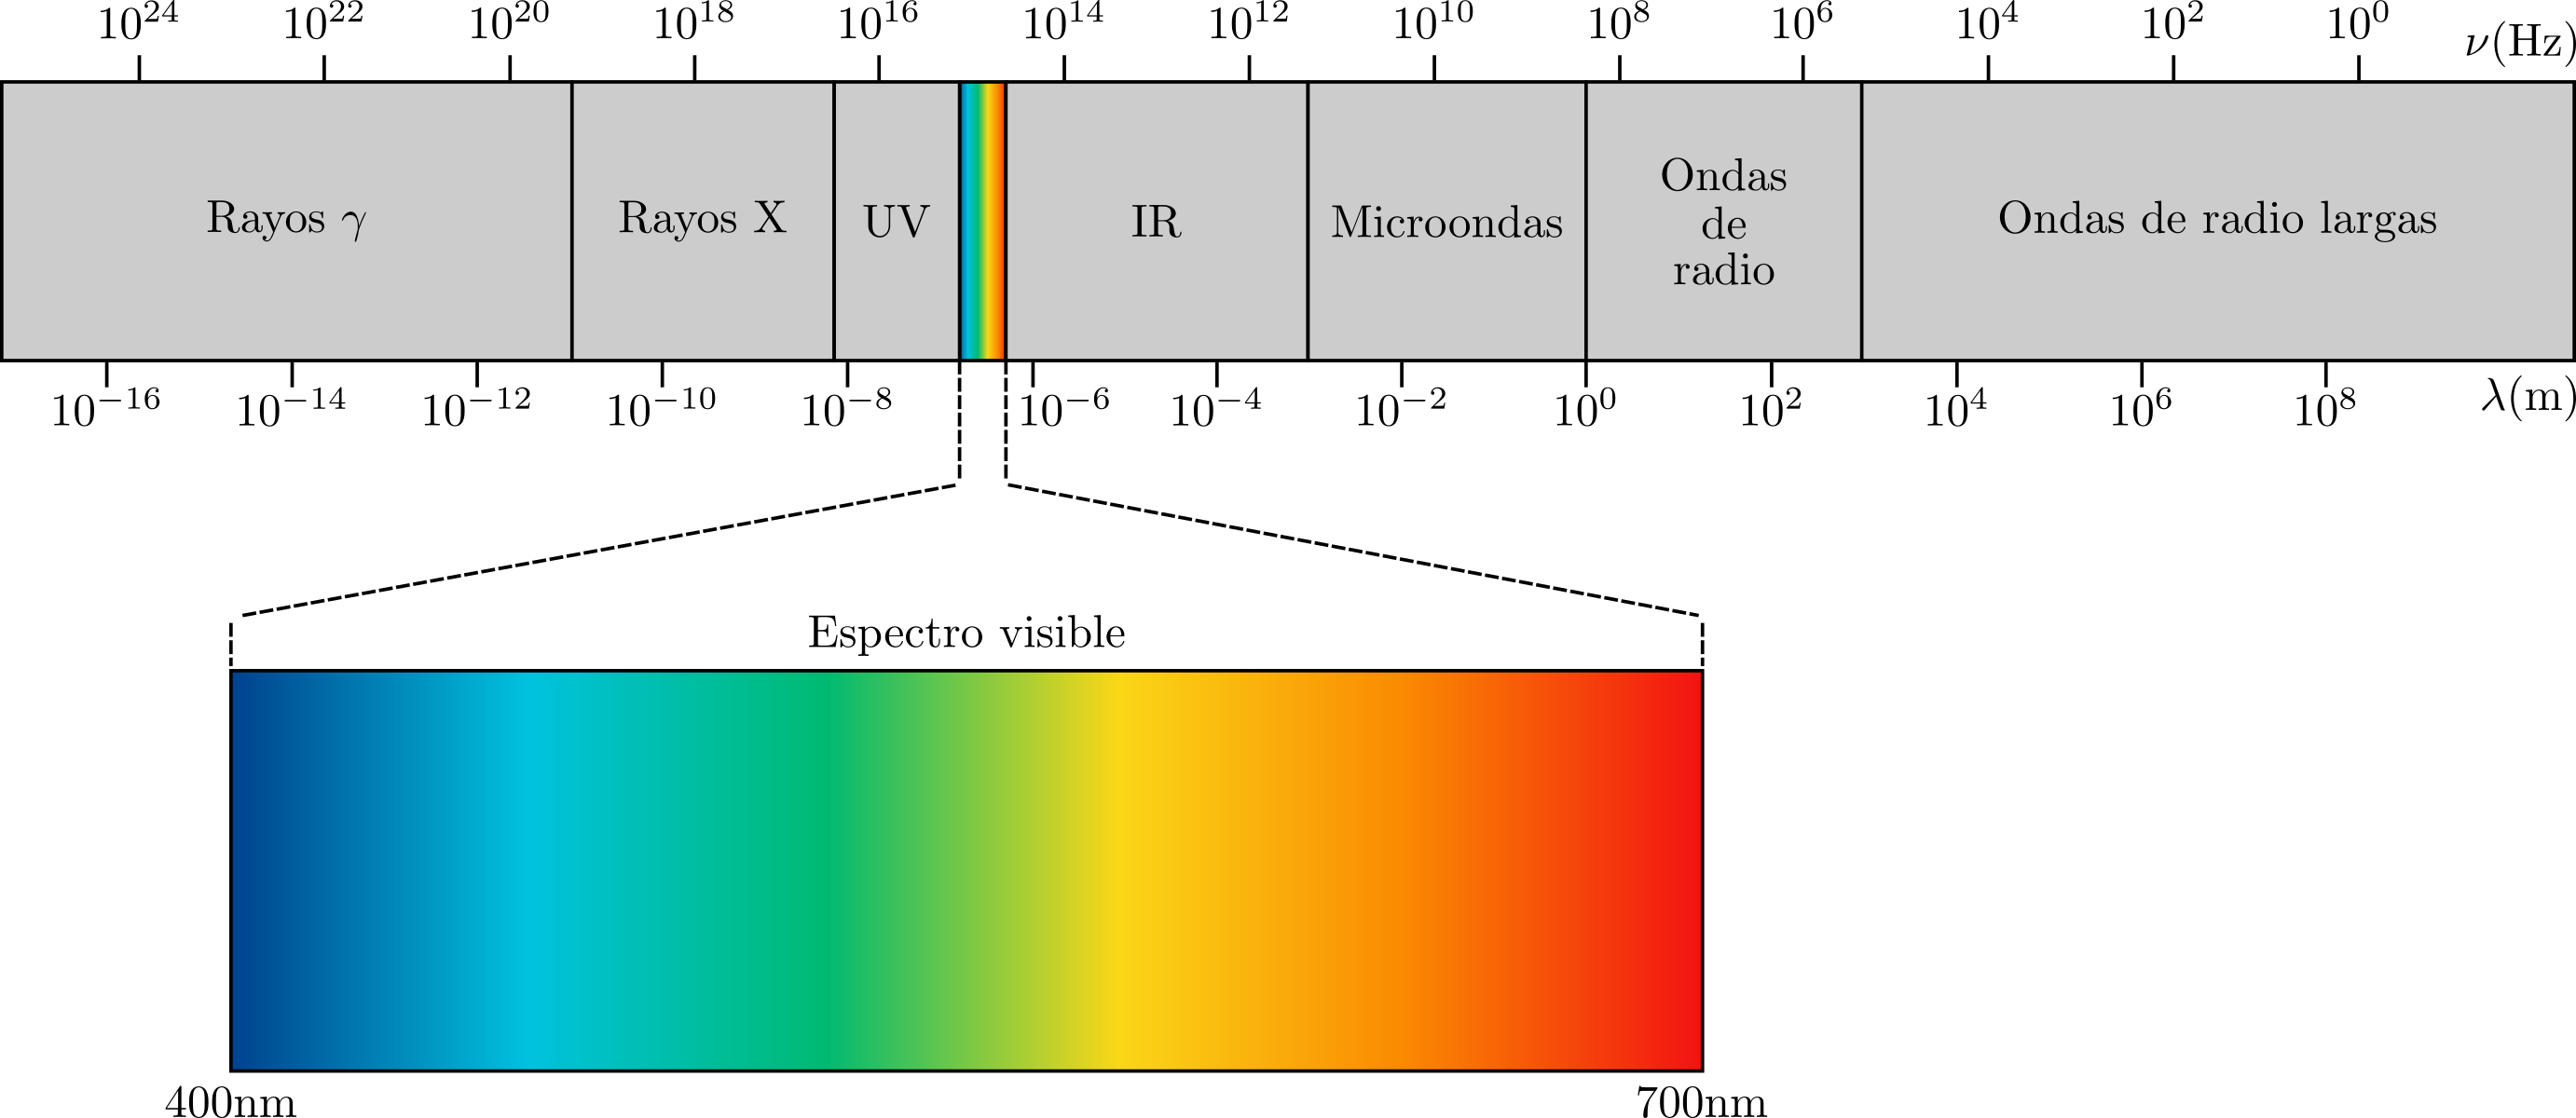
\includegraphics[width=0.8\textwidth]{espectro}
                \caption{Espectro electromagnético.}
                \label{fig:espectro}
            \end{figure}    
    
    Estas radiaciones obedecen las mismas leyes, la diferencia entre ellas radica en su longitud de onda o frecuencia, así como en la manera en que interactúan con los materiales ópticos, incluída la atmósfera \cite{Vincent}.
    
    Todos los cuerpos emiten radiación e.m  y debido al movimiento de sus átomos y moléculas se genera una temperatura en ellos. Los cuerpos con una temperatura mayor a 0K emiten radiación térmica por medio de ondas e.m. La radiación térmica es la radiación que emite un cuerpo por su temperatura \cite{Hollands}.
    
    La capacidad que tiene un cuerpo para emitir radiación está fuertemente relacionada con su capacidad de absorberla \cite{Beiser}.
    
    Una superficie ideal que absorbe toda la radiación que incide sobre él se denomina \textit{cuerpo negro} y el espectro de radiación que emite se llama \textit{radiación de cuerpo negro} \cite{Sears}.
    
    A pesar de que en la naturaleza no existe un objeto físico que pueda absorber toda la radiación incidente \cite{FUV3}, este puede representarse como un objeto hueco con una pequeña apertura donde cualquier radiación que incida en ella ingresa a la cavidad donde queda atrapada hasta que es absorbida \cite{Beiser}, \cite{FUV3}. En equilibrio térmico la radiación emitida por el cuerpo será exactamente igual a la absorbida.
    
    El cuerpo negro fue creado como una herramienta auxiliar para entender como los objetos emiten y absorben radiación.
    Hacia finales del siglo XIX la radiación de cuerpo negro ya había sido estudiada y dos leyes importantes sintetizaron los descubrimientos experimentales sobre este tema: La \textit{Ley de Stefan-Boltzmann} y la \textit{Ley de desplazamiento de Wien} \cite{FUV3}.
    
    La \textit{Ley de Stefan-Boltzmann} plantea que la intensidad de la radiación emitida por un cuerpo negro depende de su temperatura. La intensidad es proporcional a la cuarta potencia de la temperatura absoluta del cuerpo:
    
    \begin{equation}
        I = \sigma T^{4}
        \label{eq:Stefan-Boltzmann}
    \end{equation}
    donde:
    
    $T$ es la temperatura del cuerpo negro en K.
    
    $\sigma$ es la constante de Stefan-Boltzmann, $\sigma = 5.670\times10^{-8}\ W/m^{2}K^{4}$
    
    La intensidad de la radiación no se distribuye uniformemente a lo largo de todas las longitudes de onda. En cambio, su distribución puede medirse y describirse utilizando la intensidad por intervalo de longitud de onda, $I(\lambda)d\lambda$.
            \begin{figure}[hbtp]
                \centering
                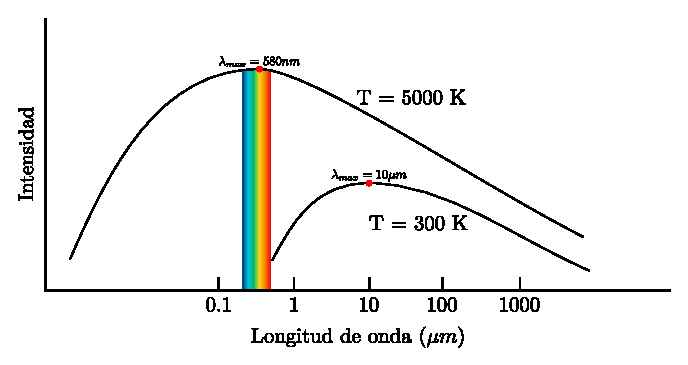
\includegraphics[width=0.8\textwidth]{intensidad_bb}
                \caption{Emitancia espectral de un cuerpo negro.}
                \label{fig:intensidad_bb}
            \end{figure}    
%    \newpage
    La Figura \ref{fig:intensidad_bb} muestra las intensidades registradas a dos temperaturas diferentes. En cada caso hay una longitud de onda específica $\lambda_{m}$ en la que la intensidad de la radiación emitida es máxima.
    
    La \textit{Ley de desplazamiento de Wien} indica que cuando la temperatura de un cuerpo negro aumenta, la longitud de onda en la que se emite la radiación máxima se desplaza hacia valores más cortos:
    
    \begin{equation}
        \lambda_{m} = \frac{2.90\times10^{-3}\ mK}{T}
        \label{eq:Wien}
    \end{equation}   
    donde:
    
    $\lambda_{m}$ es la longitud de onda en la que un cuerpo negro emite la mayor cantidad de radiación a una determinada temperatura \cite{Sears},\cite{FUV3}.
    
    De las leyes anteriores y la Figura \ref{fig:intensidad_bb} se puede deducir que la radiación UV, los rayos X y Gamma, son radiaciones más cálidas (radiaciones de alta energía), mientras que la radiación infrarroja está asociada a fenómenos con temperaturas cercanas a la temperatura ambiente \cite{Chang}, \cite{BlancoMDA}.     
    
    \section{Radiación Infrarroja} 
    La radiación infrarroja es un tipo de radiación electromagnética que cuenta con longitudes de onda mayores que las del rango visible. Se encuentra en el rango de 0.78$\mu m$ - 1$mm$ \cite{BlancoMDA}, y a su vez se divide en varias regiones las cuales se muestran en la Tabla \ref{tab:Div_IR} \cite{Rogalski}.
    
            \begin{table}[htbp]
                \caption{División de la radiación infrarroja.}
                \begin{center}
                    \resizebox{0.8\linewidth}{!}{ 
                    \begin{NiceTabular}{|l|c| }
                        \CodeBefore
                        \Body
                        \hline
                        \textbf{Region}  & \textbf{Rango de frecuencia ($\mu m$)}\\
                        \hline
                        Near infrared (NIR)   & 0.78 - 1\\
                        Short wavelength IR (SWIR)   & 1 - 3\\
                        Medium wavelength IR (MWIR) & 3 - 6\\
                        Long wavelength IR (LWIR)  & 6 - 15\\
                        Very long wavelength IR (VLWIR) & 15 - 30\\
                        Far infrared (FIR)  & 30 - 100\\
                        Submillimeter (SubMM) & 100 - 1000\\
                        \hline
                    \end{NiceTabular}
                    }
                \label{tab:Div_IR}
                \end{center}
            \end{table}
            
%            \newpage
            
Algunas de las aplicaciones de la radiación infrarroja son:
			\begin{itemize}
				\item \textbf{Visión nocturna}: Las cámaras de visión nocturna trabajan en el espectro infrarrojo para permitir la visión en la oscuridad, estas capturan la radiación térmica emitida por objetos y seres vivos.
				\item \textbf{Medicina}: Es utilizada para hallar cáncer y diabetes en el cuerpo humano.
				\item \textbf{Industria}: Inspección del estado de equipos eléctricos y mecánicos.
				\item \textbf{Conservación de energía}: Con escáneres IR se detectan pérdidas y fugas de calor en casas o industrias.
				\item \textbf{Ambientales}: Medición de la concentración de diversos gases contaminantes en la atmósfera.
				\item \textbf{Agricultura}: Monitoreo del estado de los cultivos y la salud de las plantas, la humedad del suelo y la presencia de plagas o enfermedades.
				\item \textbf{Astronomía}: Los telescopios infrarrojos permiten estudiar regiones del espacio donde se están formando estrellas.
				\item \textbf{Espectroscopía}: Usada en química y biología para identificar y analizar estructuras moleculares de sustancias.		
			\end{itemize}
\cite{Rogalski}, \cite{BlancoMDA}.

La mayoría de las aplicaciones en detección de radiación infrarroja requieren que esta se transmita a través del aire \cite{Jimenez}. La atmósfera terrestre se compone de ozono ($O_{3}$), dióxido de carbono ($CO_{2}$) y vapor de agua ($H_{2}O$). Estas moléculas bloquean algunas regiones del espectro infrarrojo, impidiendo la transmisión de la radiación IR a la atmósfera. Las longitudes de onda que no son afectadas por estas moléculas reciben el nombre de ventanas atmosféricas \cite{Rogalski}, \cite{Motilal}. En la Figura \ref{fig:atmos_window} podemos observarlas.

            \begin{figure}[hbtp]
                \centering
                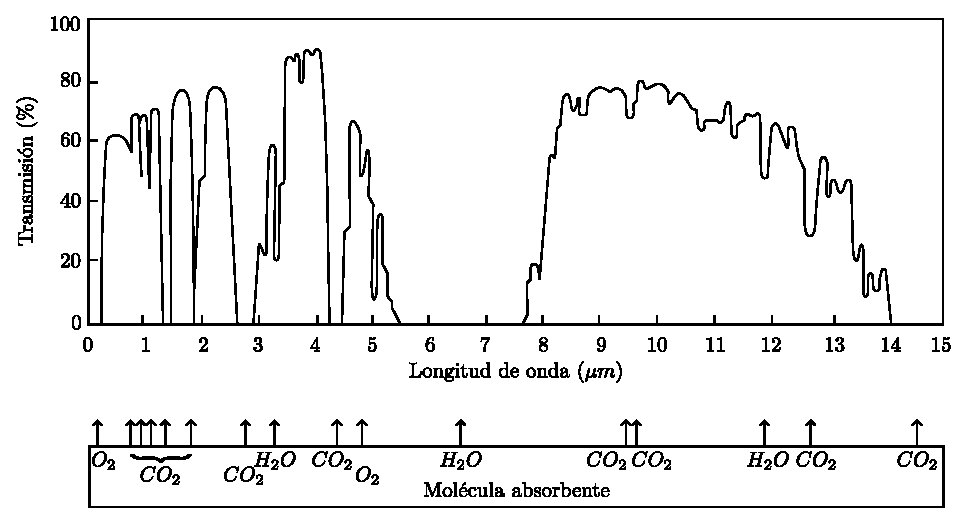
\includegraphics[width=0.8\textwidth]{atmos_window}
                \caption{Transmisión de la atmósfera.}
                \label{fig:atmos_window}
            \end{figure}



Despejando la temperatura de la ecuación \ref{eq:Wien} \cite{BlancoMDA}:
    \begin{equation}
        T_{max} = \frac{2.90\times10^{-3}\ mK}{8\mu m} = 362.5K
        \label{eq:tempmax}
    \end{equation}

    \begin{equation}
        T_{min} = \frac{2.90\times10^{-3}\ mK}{14\mu m} = 207.14K
        \label{eq:tempmin}
    \end{equation}

podemos deducir que los detectores infrarrojos que operan en la ventana de 8 - 14 $\mu m$ tienen mayor sensibilidad a la temperatura ambiente \cite{Rogalski}.

El material de fabricación y longitud de onda de operación de los detectores infrarrojos cambian de acuerdo a la aplicación en la que se desee trabajar \cite{Rogalski}.					           
     
    
    \section{Detectores Infrarrojos}
    
    Un detector infrarrojo es un dispositivo capaz de absorber parte de la energía infrarroja radiada hacia él, provocando una variación en alguna de sus propiedades eléctricas \cite{BlancoMDA}. Podemos pensar en un detector infrarrojo como un transductor, el cual convierte un tipo de señal en otra; el detector infrarrojo convierte la radiación infrarroja incidente en una señal eléctrica \cite{Vincent}.
    
    Dependiendo de la aplicación, el rango del espectro electromagnético y la temperatura en los que se desee trabajar, se debe diseñar o utilizar un detector específico que cumpla con los requerimientos, ya que cada aplicación requiere características diferentes a las demás \cite{Rogalski},\cite{BlancoMDA}.
    
    Los detectores infrarrojos se pueden clasificar en dos categorías: \textit{Detectores de fotones} y \textit{detectores térmicos}.
    
		\subsection{Detectores de fotones}
		En los detectores de fotones, la formación de pares electrón-hueco es consecuencia de la detección de radiación absorbida \cite{BlancoMDA}. En estos dispositivos, el fotón que incide sobre la superficie del material puede ser absorbido, lo que resulta en la remoción de un electrón desde la banda de valencia o desde un estado localizado dentro de la banda prohibida hasta la banda de conducción.

Generalmente, los detectores de fotones que operan a longitudes de onda de aproximadamente 3$\mu m$ requieren de un sistema de enfriamiento. Esto es necesario para prevenir la generación térmica de portadores de carga, la cual es su principal desventaja, ya que aumenta su costo y complejidad de operación. No obstante, su resolución y desempeño son bastante buenos \cite{Vincent},\cite{BlancoMDA}. 
		   
		\subsection{Detectores térmicos}
		El funcionamiento de los detectores térmicos se basa en la generación de una salida eléctrica medible como resistencia o diferencia de potencial debido al cambio de temperatura del material causado por la radiación incidente.
Estos detectores pueden funcionar a temperatura ambiente, son económicos, compactos, de bajo consumo energético y tienen una larga vida útil, pero su capacidad de detección es baja \cite{Rogalski},\cite{BlancoMDA}.
Algunos de los principales detectores térmicos infrarrojos son explicados a continuación.
		
		\subsubsection{Celda de Golay}
		La celda de Golay es un detector térmico principalmente utilizado en espectroscopía infrarroja, la celda consiste en una cámara herméticamente cerrada llena de gas y un espejo flexible. A medida que la radiación infrarroja incide, el gas se calienta y se expande, provocando que el espejo flexible se mueva. El movimiento del espejo desvía un haz de luz que incide sobre otro detector generando un cambio en su irradiancia, después esa señal es procesada \cite{Vincent},\cite{BlancoMDA}.
		\subsubsection{Bolómetros y Microbolómetros}
		Los bolómetros y microbolómetros son dispositivos que detectan la radiación infrarroja mediante el cambio en la resistencia eléctrica de un material al variar su temperatura. Conforme la resistencia absorbe calor, su temperatura aumenta y su resistencia se modifica.
Este tipo de sensores deben polarizarse con corriente o voltaje para que puedan funcionar.
Si son polarizados con corriente, el cambio de la resistencia se puede detectar y medir como un cambio de tensión, pero si se polariza con voltaje entonces se detectará como un cambio de corriente \cite{Rogalski},\cite{Vincent}.
		\subsubsection{Termopares y Termopilas}
		Los termopares y las termopilas están formados por la unión de dos conductores diferentes unidos por un extremo. Cuando la temperatura aumenta en esa unión, se genera una diferencia de potencial. Al conectar en serie varias uniones de conductores, se produce una tensión más elevada y, por lo tanto, medible \cite{Rogalski},\cite{Vincent}.
		
		\subsubsection{Detectores piroeléctricos y ferroeléctricos}
		Estos detectores pueden visualizarse como un capacitor con dos electrodos metálicos colocados perpendicularmente. Cuando un detector piroeléctrico absorbe radiación, su temperatura cambia, lo que genera una carga en el capacitor y una corriente que depende del cambio de temperatura. Si la temperatura permanece constante, la corriente será nula.

Los detectores ferroeléctricos operan bajo el mismo principio que los piroeléctricos, pero con la diferencia de que el efecto se produce mediante un campo eléctrico \cite{Rogalski}, \cite{BlancoMDA}.


En los últimos años, ha habido un creciente interés en el uso de microbolómetros para generar imágenes infrarrojas. En el ámbito médico, se han utilizado para medir la temperatura corporal \cite{Svantner2022} y, de manera innovadora, en el diagnóstico de la diabetes, mediante la captura de imágenes térmicas de la lengua \cite{WziatekKuczmik2024} o del pie \cite{Rocha2022}, permitiendo identificar variaciones térmicas que pueden indicar problemas de salud. Otra aplicación importante es en cámaras instaladas en vehículos, donde los microbolómetros se emplean para detectar personas o mascotas una vez detenido el vehículo, ayudando a prevenir accidentes ocasionados por quedar atrapados dentro \cite{Farhat2011}.


Este creciente interés se debe, en parte, a su bajo costo, peso ligero y dimensiones reducidas, que pueden ser menores a 12 $\mu$m, lo que permite una mayor cantidad de pixeles en un arreglo. Además, mientras que algunos sensores infrarrojos están limitados a resoluciones de 120$\times$84 pixeles, los microbolómetros pueden alcanzar resoluciones mucho más altas, como 1280$\times$1024 o más, obteniendo imágenes más detalladas y nítidas. Estas ventajas hacen de los microbolómetros una opción preferida en tecnologías de imágenes térmicas de alta precisión. Por este motivo, en este trabajo se desarrollará un sistema de adquisición de datos modular, que puede ser utilizado con un microbolómetro. En la siguiente tabla se presentan trabajos similares.

            \begin{table}[htbp]
                \caption{Resumen de trabajos relacionados son sistemas de lectura para detectores.}
                \begin{center}
                    \resizebox{1\linewidth}{!}{ 
                    \begin{NiceTabular}{|c|c|c|c|c|c|}
                        \CodeBefore
                        \Body
                        \hline
                        \textbf{Artículo} & \textbf{Dispositivo de implementación} & \textbf{Tecnología de detección} & \textbf{Sistema configurable} & \textbf{Interfaz gráfica} & \textbf{Arreglo máximo de detectores} \\
                        \hline
                        \multirow{2}{*}{\cite{Farhat2011}} & \multirow{2}{*}{TSK3000 Microcontrolador incluido en FPGA Altera company} & \multirow{2}{*}{Microbolómetro no refrigerado de Silicio-amorfo (a-Si)} & \multirow{2}{*}{No} & \multirow{2}{*}{Integrada} & \multirow{2}{*}{168x120} \\&  &  &  &  &  \\
                        \hline
                        \multirow{2}{*}{\cite{Sosnowski2010}} & \multirow{2}{*}{FPGA EPC2C35F672 de Altera company} & \multirow{2}{*}{UL 03 04 (comercial) Microbolómetro de Silicio-amorfo (a-Si)} & \multirow{2}{*}{No} & \multirow{2}{*}{No} & \multirow{2}{*}{384x288} \\&  &  &  &  &  \\
                        \hline
                        \multirow{2}{*}{\cite{Forsberg2015}} & \multirow{2}{*}{FPGA EPC3C40 de Altera company} & \multirow{2}{*}{Microbolómetro con pozo cuántico de Silicio (Si), Silicio-germanio (SiGe)} & \multirow{2}{*}{No} & \multirow{2}{*}{Sí} & \multirow{2}{*}{384x288} \\&  &  &  &  &  \\
                        \hline
                        \multirow{2}{*}{\cite{Vybornov2020}} & \multirow{2}{*}{Microcontrolador Cortex M3 STM32F103} & \multirow{2}{*}{Bolómetro en sustrato de Óxido de aluminio (Al2O3), Silicio (Si)} & \multirow{2}{*}{No} & \multirow{2}{*}{No} & \multirow{2}{*}{1x1} \\&  &  &  &  &  \\
                        \hline
                        \multirow{2}{*}{\cite{Xie2016}} & \multirow{2}{*}{FPGA Cyclone IV EP4CE55 de Altera company} & \multirow{2}{*}{GWR1020 IRFPA de Óxido de vanadio (VOx)} & \multirow{2}{*}{No} & \multirow{2}{*}{No} & \multirow{2}{*}{384x288} \\&  &  &  &  &  \\
                        \hline
                        \multirow{2}{*}{\cite{Feng2020}} & \multirow{2}{*}{DSP TMS320DM6467} & \multirow{2}{*}{Microbolómetro UL04371 (comercial)} & \multirow{2}{*}{No} & \multirow{2}{*}{No} & \multirow{2}{*}{160x120} \\&  &  &  &  &  \\
                        \hline
                        \multirow{2}{*}{\cite{Bayareh2018}} & \multirow{2}{*}{Raspberry Pi 2} & \multirow{2}{*}{Lepton FLIR 2.5 (comercial): Microbolómetro de VOx no refrigerado} & \multirow{2}{*}{No} & \multirow{2}{*}{Si} & \multirow{2}{*}{80x60} \\&  &  &  &  &  \\
                        \hline
                        \multirow{2}{*}{\cite{LeneroBardallo2022}} & \multirow{2}{*}{Raspberry Pi 3 B+} & \multirow{2}{*}{Lepton FLIR (comercial): Microbolómetro de VOx no refrigerado} & \multirow{2}{*}{No} & \multirow{2}{*}{No} & \multirow{2}{*}{160x120} \\&  &  &  &  &  \\
                        \hline
                        \multirow{2}{*}{\cite{Rocha2022}} & \multirow{2}{*}{Raspberry Pi} & \multirow{2}{*}{Lepton FLIR 2.5 (comercial): Microbolómetro de VOx no refrigerado} & \multirow{2}{*}{No} & \multirow{2}{*}{No} & \multirow{2}{*}{80x60} \\&  &  &  &  &  \\
                        \hline
                        \multirow{2}{*}{\cite{Javaid2020}} & \multirow{2}{*}{DROIC} & \multirow{2}{*}{Infrared pixel array} & \multirow{2}{*}{Si} & \multirow{2}{*}{Si} & \multirow{2}{*}{1024x1024} \\&  &  &  &  &  \\
                        \hline
                    \end{NiceTabular}
                    }
                \label{tab:Div_IR}
                \end{center}
            \end{table}	 					          
		
    \section{Objetivos}
	
		\subsection{Objetivo general}
			\begin{itemize}
				\item Diseño de un sistema de adquisición de datos basado en FPGA para la medición de una matriz de pixeles de un microbolómetro.
			\end{itemize}
		
		\subsection{Objetivos específicos}
			\begin{itemize}
                \item Analizar las propiedades físicas y características de los microbolómetros, así como su funcionamiento y sus diferentes circuitos de lectura con el fin de fundamentar las decisiones en el diseño del sistema.
                \item Estudiar las máquinas de estado finito (FSM) de tipo Moore y Mealy, los tipos de codificación en Verilog y las técnicas de diseño, con el fin de aplicar este conocimiento en la implementación y optimización del sistema de adquisición y procesamiento de datos.
                \item Diseñar un firmware en el lenguaje Verilog para implementar los protocolos de comunicación SPI y UART reconfigurables y robustos, que permitan adaptabilidad y confiabilidad en aplicaciones de adquisición de datos y control.
                \item Seleccionar los convertidores analógico-digital (ADC) y digital-analógico (DAC) más adecuados para el sistema de adquisición de datos y probarlos utilizando el firmware previamente diseñado.
                \item Diseñar una PCB con una matriz de 8x8 fototransistores que funcione como banco de prueba para validar el funcionamiento del sistema de adquisición de datos.
                \item Integrar los convertidores ADC y DAC, multiplexores, y la matriz de fototransistores en un sistema unificado para realizar pruebas y validar su capacidad de adquirir y procesar imágenes de manera eficiente.
			\end{itemize}
